\documentclass[UTF8,9pt]{ctexart}
\usepackage{../../template/homeworkTEMP/hw}
\setcounter{secnumdepth}{0}
\title{光学 hw} 
\begin{document}
    \maketitle
    \section{2-29, 2-30}
        \begin{center}
            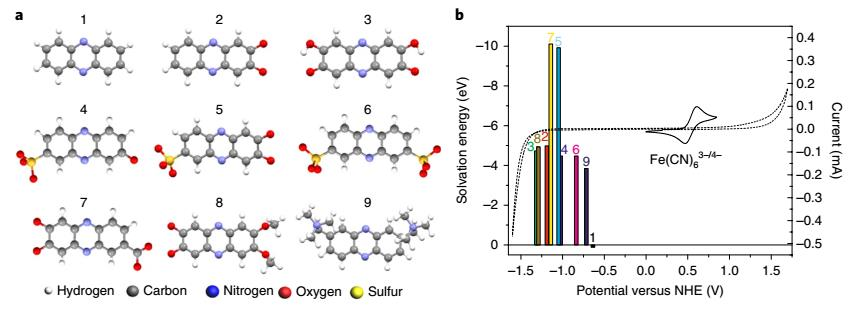
\includegraphics[scale=0.25]{3.jpg}\\
        \end{center}
    \section{2-32}
        \begin{center}
            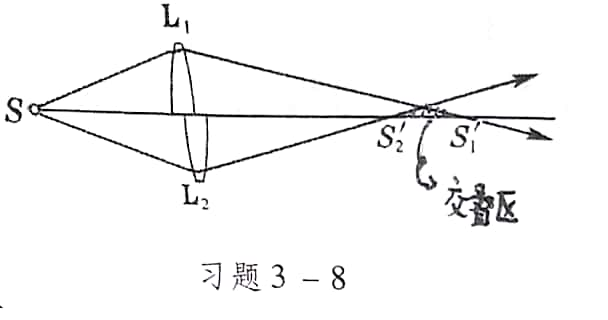
\includegraphics[scale=0.2]{2.jpg}\\
        \end{center}
    \section{2-37} 
        \begin{center}
            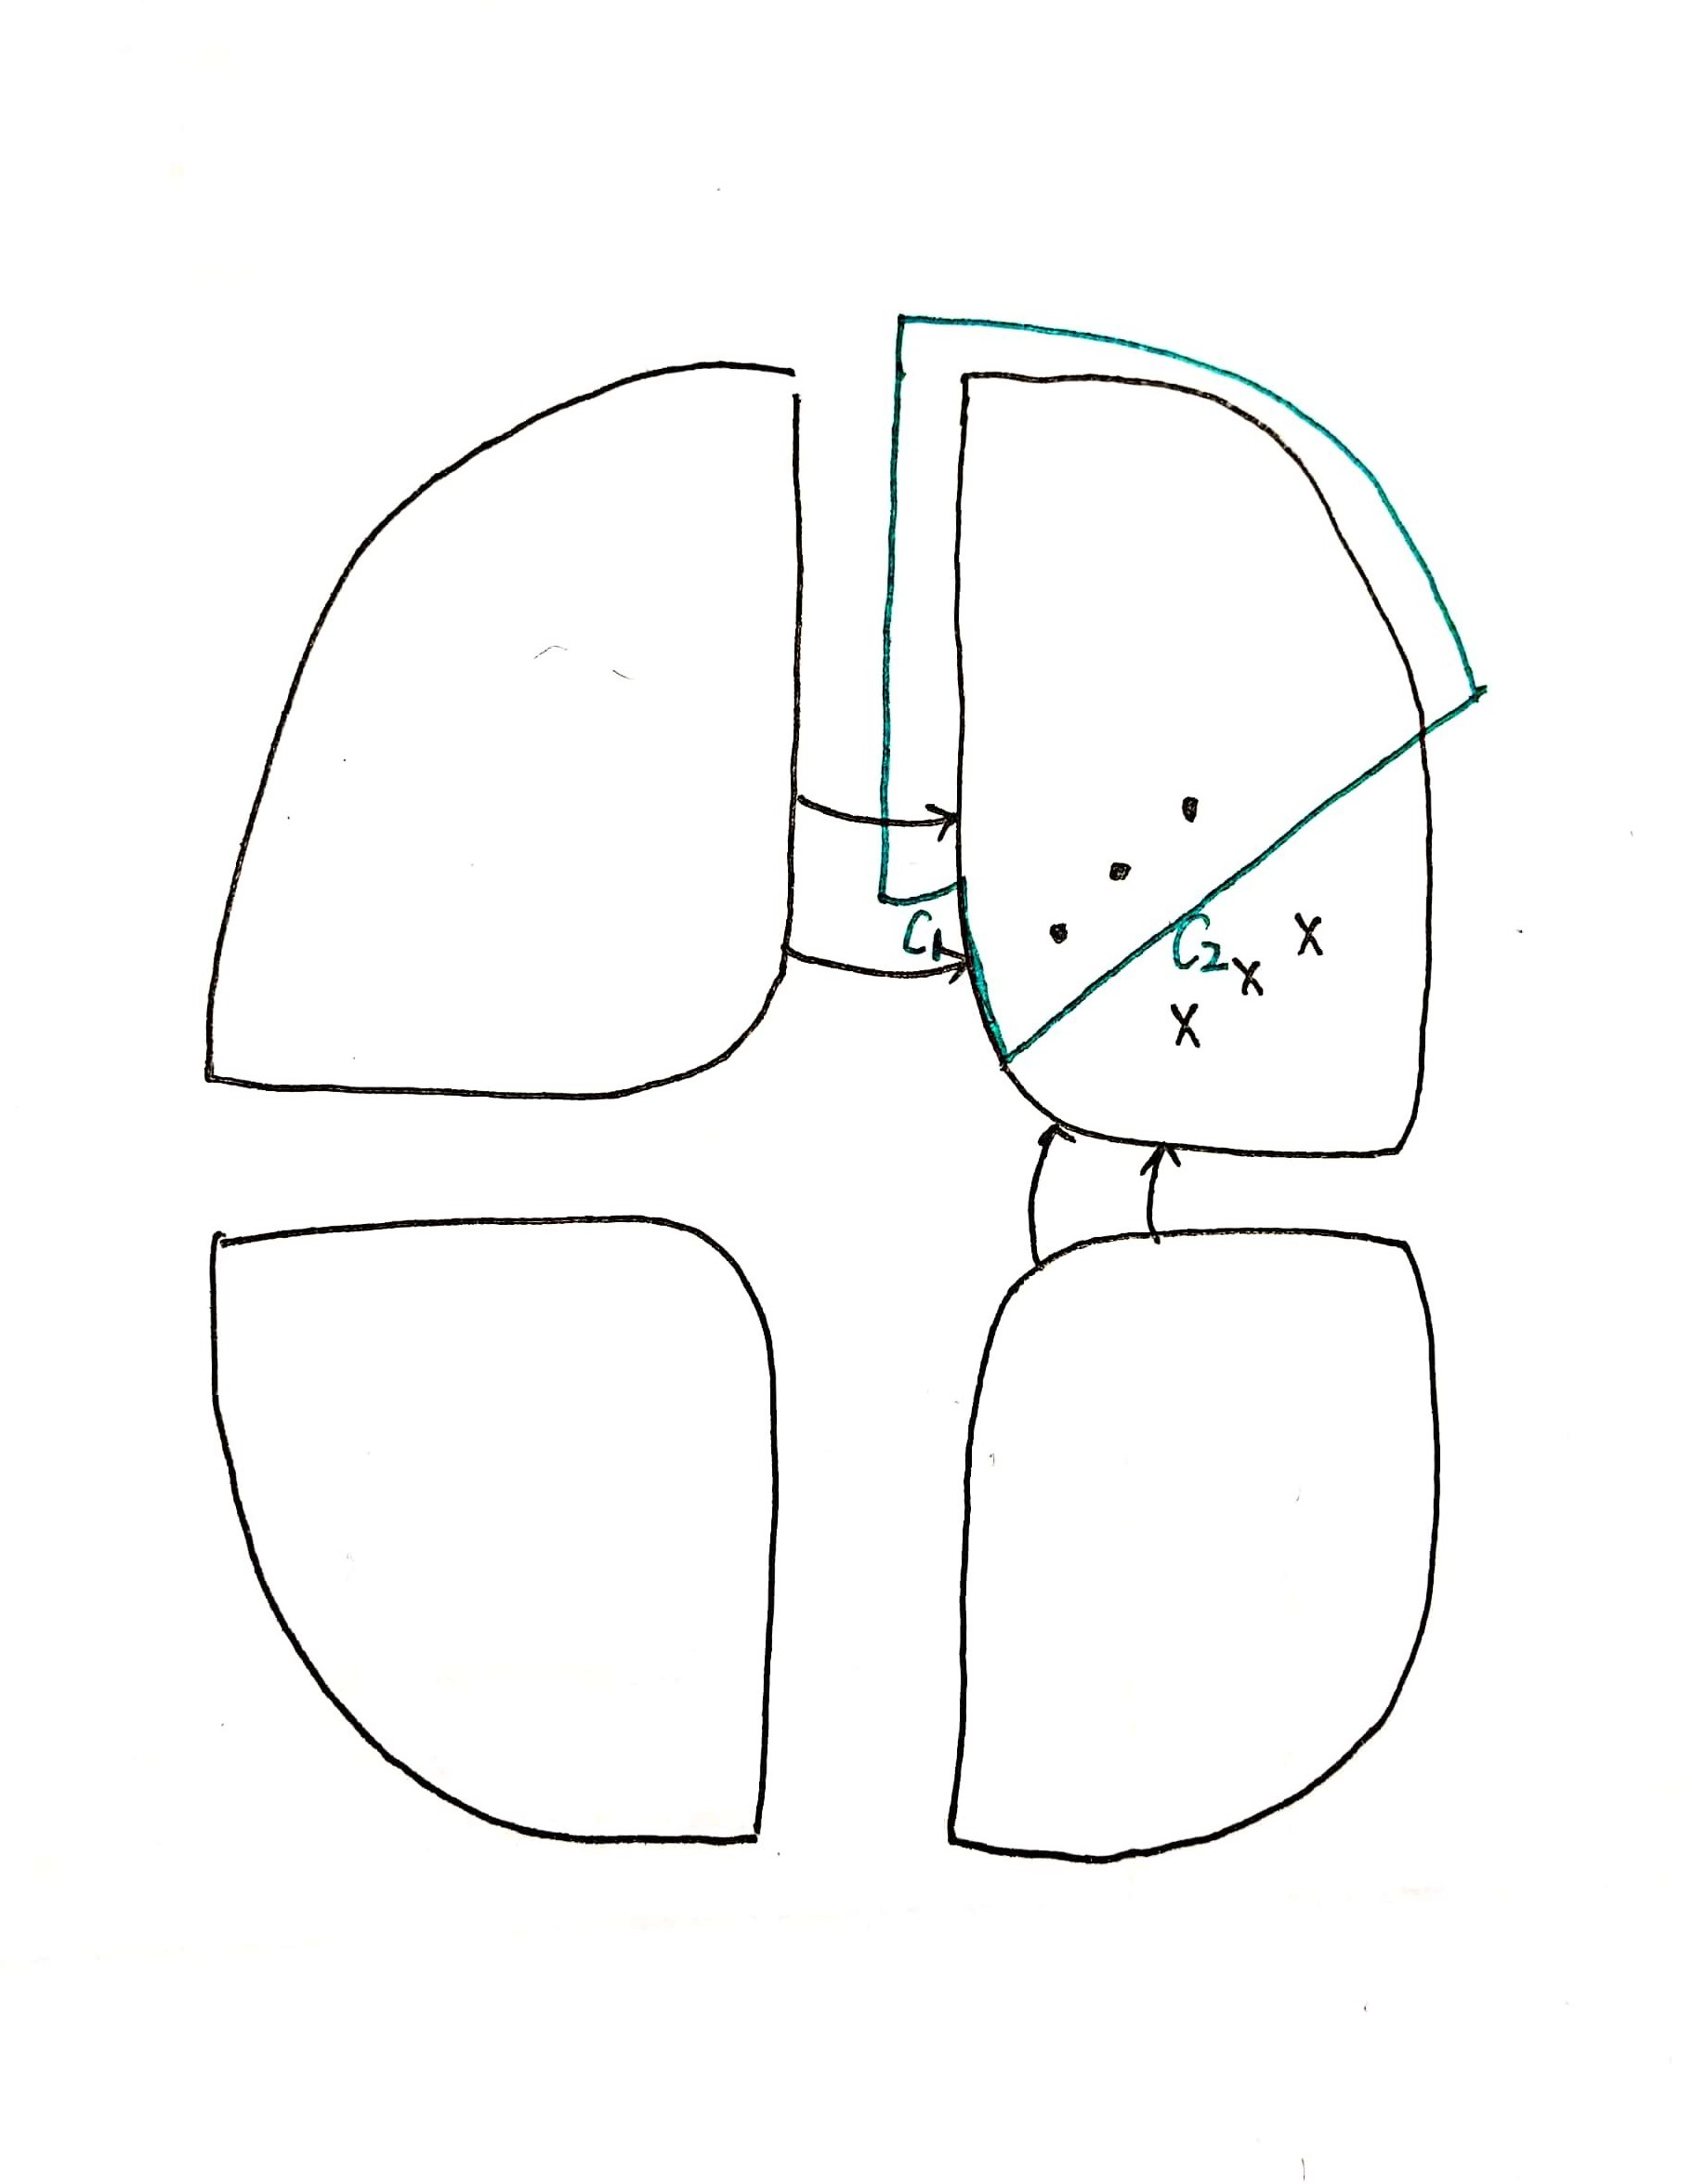
\includegraphics[scale=0.2]{1.jpg}\\
        \end{center}
        
    \section{2-40}
        \subsection*{1}
            戴上眼镜后应该能看到无穷远,即:
            $$\Phi=(\frac{1}{\infty}-\frac{1}{2.5})D=-0.4D=40\text{度}$$
        \subsection*{2}
            戴上眼镜后应该能看到明视距离0.25m,即:
            $$\Phi=(\frac{1}{0.25}-\frac{1}{1})D=3D=300\text{度}$$
    \section{2-42}
        物镜放大率:
        $$V_0=-\frac{x}{f}=-40$$
        显微镜总放大率为物镜放大率与目镜放大率之积:
        $$V_{total}=V_0\times20=-600$$
    \section{2-45}
        \begin{center}
            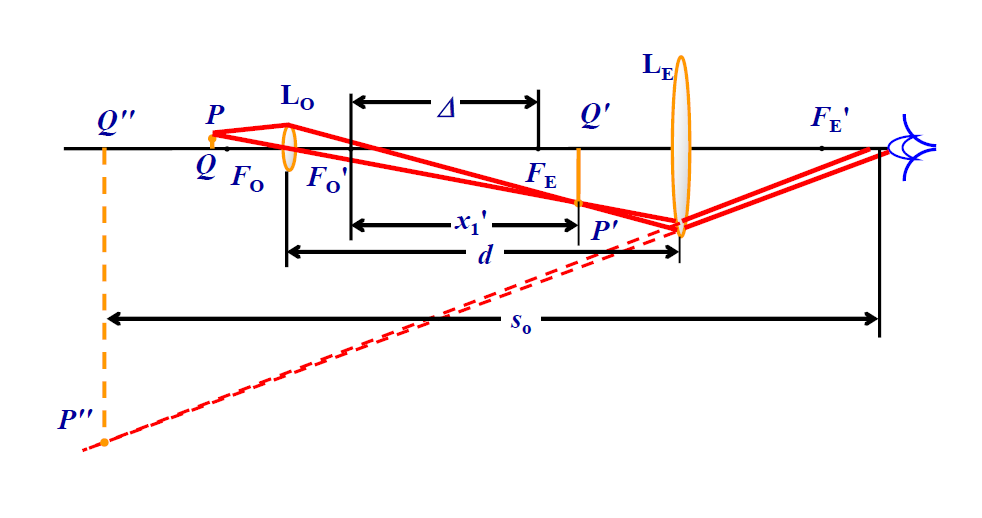
\includegraphics[scale=0.4]{4.png}\\
        \end{center}
        \subsection*{(a)开普勒型望远镜}
            其角放大率$$W=\frac{\tan(\omega')}{\tan\omega}=-3$$
            且
            $$\tan(\omega')=\frac{-y'}{f_E}\qquad \tan\omega=\frac{y'}{-f_O'}\qquad f_O'=50cm$$
            即:
            $$f_E=f_O'/3=50/3cm=16.7cm$$
            $$\Rightarrow \Phi_E=1/f_E=6m^{-1}$$
            $$d=f_O'+f_E=66.7cm$$
        \subsection*{(b)伽利略型望远镜}
            其角放大率$$W=\frac{\tan(\omega')}{\tan\omega}=-3$$
            且
            $$\tan(\omega')=\frac{-y'}{f_E}\qquad \tan\omega=\frac{y'}{f_O'}\qquad f_O'=-50cm$$
            即:
            $$f_E=f_O'/3=-50/3cm=-16.7cm$$
            $$\Rightarrow \Phi_E=1/f_E=-6m^{-1}$$
            $$d=f_O'+f_E=33.3cm$$
    \section{2-47}
        假设所求望远镜为开普勒型望远镜,则物距$s=f_O'+f_E$为两镜间隔。代入
        $$\frac{1}{s}+\frac{1}{s'}=\frac{1}{f_E}$$
        可以得到
        $$\frac{1}{f_O'+f_E}+\frac{1}{s'}=\frac{1}{f_E}$$
        $$\Rightarrow s'=\frac{f_E}{f_O'}(f_E+f_O') \simeq f_E$$
        设物镜直径$D_0$,出射光瞳直径$D'$
        放大率$$\frac{D'}{D_0}=|V|=\left|\frac{-s'}{s}\right|=\left|\frac{-\frac{f_E}{f_O}(f_E+f_O')}{f_O'+f_E}\right|$$
        对于$V$有:
        $$V=\frac{-\frac{f_E}{f_O'}(f_E+f_O)}{f_O'+f_E}=-\frac{f_E}{f_O'}$$
        即:
        $$\frac{D'}{D_0}=\left|\frac{f_E}{f_O'}\right|=1/|M|$$
        $$\Rightarrow D'=\frac{D_0}{|M|}$$
        Q.E.D.
    \section{2-49}
        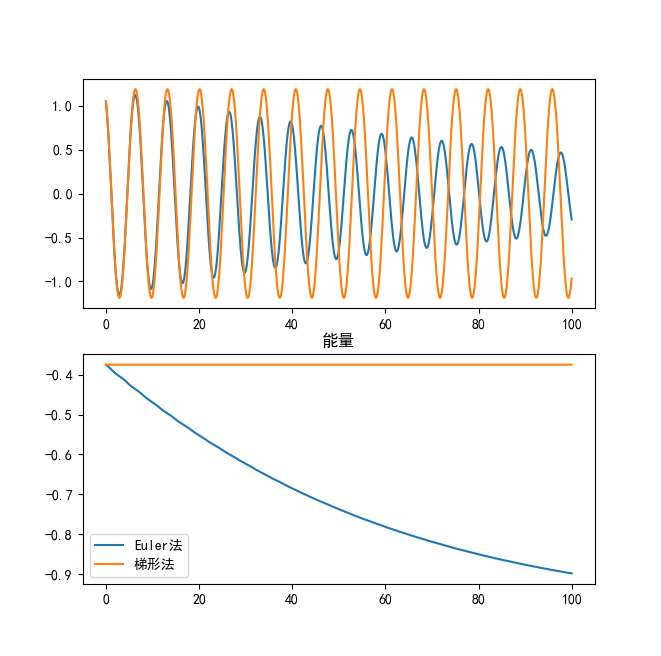
\includegraphics[scale=0.4]{5.png}\\
        \subsection*{1}
            物距$s=f_O'+f_E+\Delta$为两镜间隔。代入
            $$\frac{1}{s}+\frac{1}{s'}=\frac{1}{f_E}$$
            可以得到
            $$\frac{1}{f_O'+f_E+\Delta}+\frac{1}{s'}=\frac{1}{f_E}$$
            $$\Rightarrow s'=\frac{f_E(f_O'+f_E+\Delta)}{f_O'+\Delta}=f_E(1+\frac{f_O'}{f_O'+\Delta}) \simeq f_E$$
        \subsection*{2}
            $$\begin{array}{rl}
                M=&\f{Q'P'/f_e}{QP/s_0}=\f{Q'P'}{QP}\f{s_0}{f_e}=\f{s_0}{f_e}\f{-\Delta}{f_O'}\\
                \text{代入}V=&\f{-\Delta}{f_O'},\ f_0=nf_0'\\
                |M|=&\frac{s_0n\Delta}{f_Of_E}
            \end{array}$$
            $$\tan u_0=\frac{D_0}{2nf_O} \simeq u_0$$
            $$\f{-D'}{D_0}=V=\f{\Delta}{f_e}$$
            $$\Rightarrow \f{2s_0nu_0}{|M|}=\f{2s_0nD_0f_ef_O}{2f_Os_o\Delta n}=\f{D_0f_e}{\Delta}=D'$$
    \section{2-50}
            对于$DD$形成的入瞳$D'D'$
            $$\ff{s_0}+\ff{4a}=\ff{2a}$$
            $$\Rightarrow s_0=4a=2f_1$$
            则该入瞳半径为$r_3$\\
            对于$L_2$形成的入瞳$L_2'$
            $$\ff{s_0}+\ff{6a}=\ff{2a}$$
            $$\Rightarrow s_0=3a=\ff{2}s_0'$$
            则该入瞳半径为$r=\f{3}{2}r_3$.\\
            由几何关系,可知入瞳$D'D'$对光束限制作用最大,是真实的入瞳,该入瞳半径为$r_3$,距离$L_1$左侧$4a$。\\
            因此孔径光阑为$DD$。\\
            对于$DD$形成的出瞳$D''D''$
            $$\ff{d-l}+\ff{s_1}=\ff{a}$$
            $$\Rightarrow s_0=2a=2f_2$$
            则该出瞳距离$L_2$右侧$2a$,半径为$r_3$\\
            在孔径光阑左侧只有$L_1$限制光束,$L_1$边缘即为入射窗,视场光阑。
        \subsection*{2}
            令$K_1=\ff{r_1}-\ff{r_2}, K_2=\ff{r_2}$, 则C线和F线的光焦度分别为:
            $$P_F=(n_{F1}-1)K_1+(n_{F2}-1)K_2$$
            $$P_C=(n_{C1}-1)K_1+(n_{C2}-1)K_2$$
            由于消除相差时成像在同一点,
            $$P_F-P_C=(n_{F1}-n_{C1})K_1+(n_{F2}-n_{C2})K_2=0$$
            且焦距满足:
            $$P_D=(n_{D1}-1)K_1+(n_{D2}-1)K_2=1/100mm=10D$$
            求解上述方程,可解得:
            $$K_1 = 44.9109, K_2 = -21.2736$$
            $$\Rightarrow r_1=15.11mm, r_2=-47.01mm$$


            



\end{document}